First a few preliminary concept relevant to solving (V)PGs are introduced, specifically: existing parity game algorithms, symbolically representing sets and fixed-point theory.
\subsection{Symbolically representing sets}
A set can straightforwardly be represented by a collection containing all the elements that are in the set. We call this an \textit{explicit} representation of a set. We can also represent sets \textit{symbolically} in which case the set of elements is represented by some sort of formula. A typical way to represent a set symbolically is through a boolean formula encoded in a \textit{binary decision diagram} \cite{BDD_book,Handbook_BDD_Chapter}. For example the set $S = \{0,1,2,4,5,7 \}$ can be expressed by boolean formula:
\[ F(x_2,x_1,x_0) = (x_2 \vee \neg x_1 \vee \neg x_0) \wedge (\neg x_2 \vee \neg x_1 \vee x_0) \]
where $x_0,x_1$ and $x_2$ are boolean variables. The formula gives the following truth table:\\
\begin{center}
	\begin{tabular}{|c|c|}
		\hline 
		$\mathbf{x_2x_1x_0}$ & $\mathbf{F(x_2,x_1,x_0)}$ \\ 
		\hline 
		000 & 1 \\ 
		\hline 
		001 & 1 \\ 
		\hline 
		010 & 1 \\ 
		\hline 
		011 & 0 \\ 
		\hline 
		100 & 1 \\ 
		\hline 
		101 & 1 \\ 
		\hline 
		110 & 0 \\ 
		\hline 
		111 & 1 \\ 
		\hline 
	\end{tabular} 
\end{center}
The function $F$ defines set $S'$ in the following way: $S' = \{x_2x_1x_0\ |\ F(x_2,x_1,x_0) = 1 \}$. As we can see set $S'$ and $S$ represent the same numbers. We can perform set operations on sets represented as boolean functions by performing logical operations on the functions. For example, given boolean formula's $f$ and $g$ representing sets $V$ and $W$ the formula $f \wedge g$ represents set $V \cap W$.

Boolean functions can efficiently be represented in BDDs, for a comprehensive treatment of BDDs we refer to \cite{BDD_book,Handbook_BDD_Chapter}. We will note here that given $x$ boolean variables and two boolean functions encoded as BDDs we can perform binary operations $\vee,\wedge$ on them in $O(2^{2x})=O(m^2)$ where $m = 2^x$ is the maximum set size that can be represented by $x$ variables \cite{BDD_running_time,Handbook_BDD_Chapter}. The running time specifically depends on the size of the decision diagrams, in general if the boolean functions are simple then the size of the decision diagram is also small and operations can be performed quickly.

\subsection{Fixed-point theory} 
A fixed-point of a function is an element in the domain of that function such that the function maps to itself for that element. Fixed-point theory goes hand in hand with lattice theory which we introduce first.
\subsubsection{Lattices}
We introduce definitions for ordering and lattices taken from \cite{birkhoff1940lattice}.
\begin{definition}
	A partial order is a binary relation $x \leq y$ on set $S$ where for all $x,y,z \in S$ we have:
	\begin{itemize}
		\item $x \leq x$. (Reflexive)
		\item If $x \leq y$ and $y \leq x$, then $x=y$. (Antisymmetric)
		\item If $x \leq y$ and $y \leq z$, then $x \leq z$. (Transitive)
	\end{itemize}
\end{definition}

\begin{definition}
	A partially ordered set is a set $S$ and a partial order $\leq$ for that set, we denote a partially ordered set by $\langle S, \leq \rangle$.
\end{definition}

\begin{definition}
	Given partially ordered set $\langle P,\leq \rangle$ and subset $X \subseteq P$. An upper bound to $X$ is an element $a \in P$ such that $x \leq a$ for every $x\in X$. A least upper bound to $X$ is an upper bound $a \in P$ such every other upper bound is larger or equal to $a$.
	
	The term least upper bound is synonymous with the term supremum.
\end{definition}
\begin{definition}
	Given partially ordered set $\langle P,\leq \rangle$ and subset $X \subseteq P$. A lower bound to $X$ is an element $a \in P$ such that $a \leq x$ for every $x\in X$. A greatest lower bound to $X$ is a lower bound $a \in P$ such that every other lower bound is smaller or equal to $a$.
	
	The term greatest lower bound is synonymous with the term infimum.
\end{definition}

\begin{definition}
	A lattice is a partially ordered set where any two of its elements have a supremum and an infimum.
\end{definition}

\begin{definition}
	A complete lattice is a partially ordered set in which every subset has a supremum and an infimum.
\end{definition}

\begin{definition}
	A function $f : D \rightarrow D'$ is monotonic, also called order preserving, if for all $x \in D$ and $y \in D$ it holds that if $x \leq y$ then $f(x) \leq f(y)$.
\end{definition}
\subsubsection{Fixed-points}
Fixed-points are formally defined as follows:
\begin{definition}
	Given function $f : D \rightarrow D$ the value $x \in D$ is a fixed point for $f$ if and only if $f(x) = x$.
\end{definition}
\begin{definition}
	Given function $f : D \rightarrow D$ the value $x \in D$ is the least fixed point for $f$ if and only if $x$ is a fixed point for $f$ and every other fixed point for $f$ is greater or equal to $x$.
\end{definition}
\begin{definition}
	Given function $f : D \rightarrow D$ the value $x \in D$ is the greatest fixed point for $f$ if and only if $x$ is a fixed point for $f$ and every other fixed point for $f$ is less or equal to $x$.
\end{definition}
The Knaster-Tarski theorem states that least and greatest fixed points exist for some domain and function given that a few conditions hold.
The theorem, as written down by Tarski \cite{tarski1955}, states:
\begin{theorem}[Knaster-Tarski\cite{tarski1955}]
	\label{the_knaster_tarski}
	Let
	\begin{itemize}
		\item $\langle A, \leq \rangle$ be a complete lattice,
		\item $f$ be an increasing function on $A$ to $A$,
		\item $P$ be the set of all fixpoints of f.
	\end{itemize}
	Then the set $P$ is not empty and the system $\langle P, \leq \rangle$ is a complete lattice; in particular we have 
	\[ \sup P = \sup \{ x\ |\ f(x) \geq x \} \in P \]
	and
	\[ \inf P = \inf \{ x\ |\ f(x) \leq x \} \in P \]
\end{theorem}
\subsection{Parity game algorithms}
We inspect two existing parity game algorithms which are used in the collective VPG algorithms. First Zielonka's recursive algorithm which is well studied and generally considered to be one of the best performing parity game algorithm \cite{Oink,SolvingPGInPractice}. We also inspect the fixed-point iteration algorithm which tends to perform well for model-checking problems with a low number of distinct priorities \cite{BDDSolvingPG}.

\subsubsection{Zielonka's recursive algorithm}
First we consider Zielonka's recursive algorithm, created from the constructive proof given in \cite{ZIELONKA1998135}, which solves total PGs. Pseudo code is presented in algorithm \ref{alg_zlnk_org}. Zielonka's recursive algorithm has a worst-case time complexity of $O(e*n^d)$.
\begin{algorithm}
	\caption{$\textsc{RecursivePG}(\textit{PG } G = (V,V_0,V_1, E, \Omega))$}
	\label{alg_zlnk_org}
	\begin{algorithmic}[1]
		\State $m \gets \min\{ \Omega(v)\ |\ v \in V\}$
		\State $h \gets\max\{ \Omega(v)\ |\ v \in V\}$
		\If{$h = m$ or $V = \emptyset$}
		\If{$h$ is even or $V = \emptyset$}
		\State \Return $(V,\emptyset)$
		\Else
		\State \Return $(\emptyset, V)$
		\EndIf
		\EndIf
		\State $\alpha \gets 0$ if $h$ is even and $1$ otherwise
		\State $U \gets \{v \in V\ |\ \Omega(v) = h\}$
		\State $A \gets \alpha\textit{-Attr}(G, U)$
		\State $(W_0', W_1') \gets \textsc{RecursivePG}(G \backslash A)$
		\If{$W_{\overline{\alpha}}' =\emptyset$}
		\State $W_\alpha \gets A \cup W_\alpha'$
		\State $W_{\overline{\alpha}} \gets \emptyset$
		\Else
		\State $B \gets \overline{\alpha}\textit{-Attr}(G,W_{\overline{\alpha}}')$
		\State $(W_0'', W_1'') \gets \textsc{RecursivePG}(G \backslash B)$
		\State $W_\alpha \gets W_\alpha''$
		\State $W_{\overline{\alpha}} \gets W_{\overline{\alpha}}'' \cup B$
		\EndIf
		\State \Return $(W_0, W_1)$
	\end{algorithmic}
\end{algorithm}

The algorithm works for solving $G$ by taking the set of vertices with the highest priority and choosing player $\alpha$ such that $\alpha$ has the same parity as the highest priority. Next the algorithm finds all the vertices such that player $\alpha$ can force the play to one of these high priority vertices. Next this set of vertices is removed from the game and the resulting subgame is solved recursively. This subgame returns winning sets $W'_0$ and $W'_1$. Vertices in set $W'_{\overline{\alpha}}$ are won by player $\overline{\alpha}$ in the subgame but are also won by player $\overline{\alpha}$ in $G$. The algorithm tries to find all the vertices in $G$ such that player $\overline{\alpha}$ can force the play to a vertex in $W'_{\overline{\alpha}}$ and therefore winning the game. We now have a set of vertices that are definitely won by player $\overline{\alpha}$ in game $G$. In the rest of the game player $\alpha$ can keep the play from $W'_{\overline{\alpha}}$ so the algorithm solves the rest of the game recursively to find the complete winning sets for game $G$.

A complete explanation of the algorithm can be found in \cite{ZIELONKA1998135}, we do introduce definitions for the attractor set and for subgames. 

An attractor set is a set of vertices $A \subseteq V$ calculated for player $\alpha$ given set $U \subseteq V$ where player $\alpha$ has a strategy to force the play starting in any vertex in $A \backslash U$ to a vertex in $U$.

\begin{definition}\cite{ZIELONKA1998135}
	\label{def_attr}Given parity game $G = (V,V_0,V_1,E,\Omega)$ and a non-empty set $U \subseteq V$ we define $\alpha\textit{-Attr}(G,U)$ such that
	\[U_0 = U \]
	For $i \geq 0$:
	\begin{align*}
	U_{i+1} = U_i\cup
	&\{v \in V_\alpha\ |\ \exists v' \in V : v' \in U_i \wedge (v,v') \in E \}\\
	\cup &\{v \in V_{\overline{\alpha}}\ |\ \forall v' \in V :(v,v') \in E \implies v' \in U_i \}
	\end{align*}
	Finally:
	\[\alpha\textit{-Attr}(G,U) = \bigcup_{i \geq 0} U_i \]
\end{definition}

\begin{figure}
	\centering
	\begin{subfigure}{1\textwidth}
		\centering
		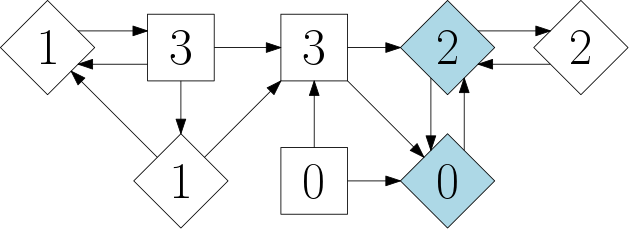
\includegraphics[scale=0.4]{Examples/Attr/Attr0}
		\caption{Set $U = U_0$}
	\end{subfigure}\\
	\begin{subfigure}{1\textwidth}
		\centering
		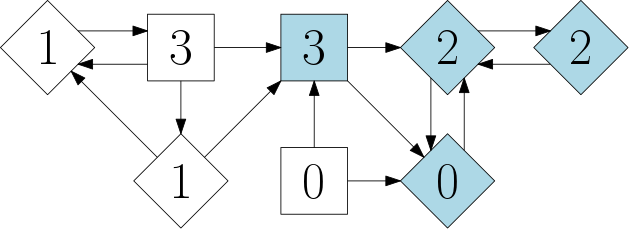
\includegraphics[scale=0.4]{Examples/Attr/Attr1}
		\caption{Set $U_1$}
	\end{subfigure}\\
	\begin{subfigure}{1\textwidth}
		\centering
		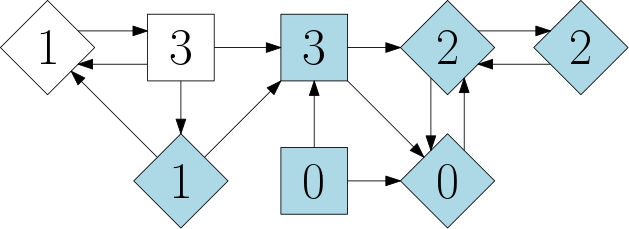
\includegraphics[scale=0.4]{Examples/Attr/Attr2}
		\caption{Set $U_2 = 0\textit{-Attr}(G,U)$}
	\end{subfigure}
	\caption{Game $G$ showing the attractor calculation for $0\textit{-Attr}(G,U)$}
	\label{fig:AttrCalcExample}
\end{figure}
Figure \ref{fig:AttrCalcExample} shows an example parity game in which an attractor set is calculated for player $0$. For set $U_2$ no more vertices can be attracted so we found the complete attractor set.

The algorithm also creates subgames, where a set of vertices is removed from a parity game to create a new parity game.

\begin{definition}\cite{ZIELONKA1998135}
	\label{def_org_subgame}
	Given a parity game $G = (V,V_0,V_1, E,\Omega)$ and $U \subseteq V$ we define the subgame $G \backslash U$ to be the game $(V', V_0', V_1', E', \Omega)$ with:
	\begin{itemize}
		\item $V' = V \backslash U$,
		\item $V_0' = V_0 \cap V'$,
		\item $V_1' = V_1 \cap V'$ and
		\item $E' = E \cap (V' \times V')$.
	\end{itemize}
\end{definition}

Note that a subgame is not necessarily total, however the recursive algorithm always creates subgames that are total (shown in \cite{ZIELONKA1998135}).

\subsubsection{Fixed-point iteration algorithm}
Parity games can be solved by solving an alternating fixed-point formula, as shown in \cite{WALUKIEWICZ2002311}. We will consider PG $G = (V,V_0,V_1, E, \Omega)$ with $d$ distinct priorities. We can apply \textit{priority compression} to make sure every priority in $G$ maps to a value in $\{0,\dots,d-1\}$ or $\{1, \dots, d\}$ \cite{SolvingInPractice,FPITE}. We assume without loss of generality that the priorities map to $\{0,\dots,d-1\}$ and that $d-1$ is even. 

Consider the following formula
\[ S(G = (V,V_0,V_1,E,\Omega)) = \nu Z_{d-1}. \mu Z_{d-2}. \dots . \nu Z_0. F_0(Z_{d-1},\dots,Z_0) \]
with
\[ F_0(Z_{d-1},\dots,Z_0) = \{ v \in V_0\ |\ \exists_{w\in V} (v,w) \in E \wedge Z_{\Omega(w)} \} \cup \{ v \in V_1\ |\ \forall_{w\in V} (v,w) \in E \implies Z_{\Omega(w)} \} \]
where $Z_i \subseteq V$. The formula $\nu X. f(X)$ solves the greatest fixed-point of $X$ in $f$, similarly $\mu X.f(X)$ solves the least fixed-point of $X$ in $f$.

To understand the formula we consider sub-formula $\nu Z_0. F_0(Z_{d-1},\dots,Z_0)$. This formula holds for vertices from which player $0$ can either force the play into a node with priority $i > 0$ for which $Z_i$ holds or the player can stay in vertices with priority $0$ indefinitely. The formula $\mu Z_0. F_0(Z_{d-1},\dots,Z_0)$ holds for vertices from which player $0$ can force the play into a node with priority $i > 0$, for which $Z_i$ holds in finitely many steps. By alternating fixed-points the formula allows infinitely many stays in even vertices and finitely many stays in odd vertices. For an extensive treatment we refer to \cite{WALUKIEWICZ2002311}.

We further inspect formula $S$. Given game $G$, consider the following subformula's:
\[ S^{d-1}(Z_{d-1}) = \mu Z_{d-2}.S^{d-2}(Z_{d-2})\]
\[ S^{d-2}(Z_{d-2}) = \nu Z_{d-3}.S^{d-3}(Z_{d-3})\]
\begin{center}
	\dots
\end{center}
\[ S^{0}(Z_0) = F_0(Z_{d-1},\dots,Z_0)\]
The fixed-point variables are all elements of $2^V$, therefore we have for every subformula the following type:
\[ S^i(Z_i) : 2^V \rightarrow 2^V \]
Furthermore, since $V$ is finite, the partially ordered set $\langle 2^V, \subseteq \rangle$ is a complete lattice.

Finally every subformula is $S^i(Z_i)$ is monotonic, ie. if $S^i(Z_i) \geq S^i(Z_i')$ then $Z_i \geq Z_i'$.

Fixed-point formula's can be solved by fixed-point iteration. As shown in \cite{Emerson:1986:MCP:900378} we can calculate $\mu X.f(X)$, where $f$ is monotonic in $X$ and $X \in 2^V$, by iterating $X$:
\[ \mu X.f(X) = \bigcup_{i \geq 0} X^i \]
where $X^i = f(X^{i-1})$ for $i > 0$ and $X^0 \subseteq \mu X.f(X)$. So picking the smallest value possible for $X_0$ will always correctly calculate $\mu X. f(X)$.

Similarly we can calculate fixed-point $\nu X.f(X)$ when $f$ is monotonic in $X$ by iterating $X$.
\[ \nu X.f(X) = \bigcap_{i \geq 0} X^i \]
where $X^i = f(X^{i-1})$ for $i > 0$ and $X^0 \supseteq \nu X.f(X)$. So picking the largest value possible for $X_0$ will always correctly calculate $\nu X. f(X)$.

Since every subformula is monotonic and maps from a value in $2^V$ to another value in $2^V$ we can apply fixed-point iteration to solve the subformula's, we choose initial values $\emptyset$ for least fixed-point variables and $V$ for greatest fixed-point variables.

An algorithm to perform the iteration is presented in \cite{FPITE} and shown in algorithm \ref{alg_FPITEorg}. This algorithm has a worst-case time complexity of $O(e * n ^d)$.
\begin{algorithm}
	\caption{Fixed-point iteration}
	\label{alg_FPITEorg}
	\begin{multicols}{2}
		\begin{algorithmic}[1]
			\Function{FPIter}{$G = (V, V_0, V_1, E, \Omega)$}
			\For{$i \gets d-1,\dots,0$}
			\State $\textsc{Init}(i)$
			\EndFor
			\Repeat
			\State $Z_0'\gets Z_0$
			\State $Z_0 \gets \textsc{Diamond}() \cup \textsc{Box}()$
			\State $i \gets 0$
			\While{$Z_i=Z_i' \wedge i < d-1$}
			\State $i \gets i+1$
			\State $Z_i' \gets Z_i$
			\State $Z_i \gets Z_{i-1}$
			\State $\textsc{Init}(i-1)$
			\EndWhile
			\Until{$i = d-1 \wedge Z_{d-1} = Z_{d-1}'$}
			\State \Return $(Z_{d-1},V\backslash Z_{d-1})$
			\EndFunction
		\end{algorithmic}\bigskip\bigskip
		\begin{algorithmic}[1]
			\Function{Init}{$i$}
			\State $Z_i \gets \emptyset$ if $i$ is odd, $V$ otherwise
			\EndFunction
		\end{algorithmic}\bigskip
		\begin{algorithmic}[1]
			\Function{Diamond}{}
			\State \Return $\{ v \in V_0\ |\ \exists_{w\in V} (v,w) \in E \wedge w \in Z_{\Omega(w)}\}$
			\EndFunction
		\end{algorithmic}\bigskip
		\begin{algorithmic}[1]
			\Function{Box}{}
			\State \Return $\{ v \in V_1\ |\ \forall_{w\in V} (v,w) \in E \implies w \in Z_{\Omega(w)}\}$
			\EndFunction
		\end{algorithmic}
	\end{multicols}
\end{algorithm}

\subsection{Locally solving parity games}
Parity games can be solved \textit{globally} or \textit{locally}; globally solving a parity game means that for every vertex in the game it is determined who the winner is. Locally solving a parity game means that for a specific vertex in the game it is determined who the winner is. For some applications of parity games, including model checking, there is a specific vertex that needs to be solved to solve the model checking problem so locally solving the parity game is sufficient for solving the original problem.

Most parity game algorithms are concerned with global solving, when talking about solving a PG we talk about globally solving it unless stated otherwise. 